\documentclass[a4paper, 10pt]{article}

\usepackage{graphicx}
\usepackage{makeidx}
\usepackage{formular}
\usepackage{listings}
\usepackage[utf8]{inputenc}
\usepackage[dvipsnames]{xcolor}

\usepackage{mdframed}
\usepackage{multicol}
\usepackage{hyperref}
\usepackage{geometry}
\usepackage{mdframed}
\usepackage{listings}

\geometry{hmargin=2.5cm, lmargin=3cm, rmargin=2cm}

\title{Notes and Logbook}
\author{Sinan DAROUKH}
\date{4th May 2019}

\begin{document}

\begin{titlepage}
\maketitle
\end{titlepage}

\tableofcontents
\newpage

\section{WinCC OA \&  The JCOP Framework ?}
\subsection{What is WINCC-OA ?}
WinCC-OA is the Supervisory Control And Data Acquisition (aka SCADA) system chosen by JCOP.
WinCC-OA aims is mainly to control and acquire data from the sensors from reals controls on experiments.
PVSS was a SCADA system, made by ETM. Siemens now owns ETM and rebranded PVSS as WinCC-OA, but it's still the same tool.
It's a tool for building SCADA applications

\subsection{What is JCOP ?}
JCOP stands for Joint COntrols Project which is a collaboration between the LHC experiments, the PH Departement and EN-ICE, the Controls Group in the Engineering Departement. JCOP aims to reduce the overall manpower cost required to produce and run the experiment control systems.
The JCOP Framework provides all the components required for WinCC-OA tool. Basically, it's a layer of software components.

\subsection{What is FSM ?}
FSM stands for Final State Machine, it's abstract representation of your experiment.


\subsection{Exercice \#1}
I have been trying http access into PMON with devwinccweb02:4999 on the lbts machine, it works fine.
However I do not understand how the layout thing work so I better ask Luis.

\subsection{Exercice \#2}
I have done the exercice 2, slide 127 is useful to understand the architecture of DataPoint (DP)
Note to self : Make a scheme about DPT, DP and DPE
All the process to create a DataPoint Type, instanciate a DataPoint is in here.

\subsection{Exercice \#3}
Original value from the PARA editor :\_original..\_value
PARA is very useful to debug and initialize :\_original..\_value
Learn about callback function, how to initialize components, also how to generate script using the wizard.

\subsection{Exercice \#4}

Slide 165 : A note on dynamic arrays
dyn\_int, dyn\_errClass, dyn\_float are just dynamic arrays of int, errClass, floats, etc \dots 
Length of the dynamic array can be check using dynlen() function.
errClass is a class dealing with special WinCC err.

Slide 166 : anytype/mixed types
anytype type enables developers to write functions that accept parameters or arbitrary type (very simple generic programming). Once an anytype variable is written to, it starts to behave as if it was of a type of the literal/variable that was assigned to it.

Pro-tips : Use const references, to avoid needless copying of variables in callback functions

\subsection{Extending Exercise \#4}
Interesting point of view of why we should not try to save space doing interface but caring about color blind people. Slide 187 : Basic DP access functions
dpGet() - get the value of a datapoint config attribute once.
dpConnect() - register a callback to be executed whenever a datapoint config attribut changes.
dpSet()/dpSetWait() - set the value of a datapoint config attribute.

\paragraph{}
Check also for dpQuery(), dpDelete(), etc\dots

\paragraph{}
Slide 188 : Performance
dpSetWait() - set around ~1000 datapoints in a single function call.
dpGet() - request values of as many datapoints as possible (pratical) in a single function call.

Executing them for a single datapoint, is one the biggest performance killers in WinCC OA ! Warning !

Slide 194 : More Aesthitics (Aesthitics standards to check)

Slide 197 : Do not add computations, e.g. comparing voltage levels in panel code instead put those functions in CONTROL libraries. UI should only do UI stuffs.

Slide 203 : Rewiew - Storage of values
There are 3 different “places” where we can storevalues.\\
You need to distinguish:
\begin{itemize}
    \item A number in a data point element.\\
DPs (and hence DPEs) are held in the Event Manager process’s memory space.
    \item A number in a widget on a panel.\\
Widgets are held in a User Interface Manager.
    \item A CONTROL variable in a script behind a widget.
\end{itemize}

Remember to name every widget, else you won't be able to access them from other widgets panel.
(Check Slide for conventionnal names 205)

DP Name Syntax in Script (Slide 208 - Good one, very important)

\section{WinCC OA \&  The JCOP Framework Course - Part 2}
\subsection{Exercice \#5}
Slide 10 : Concept of a reference panel which can be useful and time-saver.
Draw it once, but instanciate it many times.

To make a "normal" panel as a reference panel, we have edit the previous script we made and make them more generic with \$parameters.

What happens if you change the reference panel and then re-open the parent panel ?
Changes are applied to the parent panel.

How could you change it again to require that the user must supply a system name (dist\_nn:) each time he makes a new panel instance?
By using the same process as the \$parameters for the distro.

\subsection{Properties}
Performance penalty
Defined in the ScopeLib of each panels.
Cleaner way to pass parameters to the reference panel.

\subsection{Exercice \#5 - Scripts and CTRL Manager}
Scripts are contained in the Script folder, they run in the background, we need to associate them a CTRL manager to run.
If we edit a script, which already associated with a CTRL manager, we need to restart the CTRL manager.

Slides 57-61 ARE IMPORTANT

\subsection{Exercice \#6 - Debugging Tips}
\begin{itemize}
    \item Look the logviewer
    \item Check Manager Status
    \item Use PARA
    \item Use DebugTN() and DebugFTN()
\end{itemize}
DebugTN("") : DebugTN(“Entering with pressure=” + pressure);\\
DebugFTN(""): DebugFTN(“myDebugFlag","Custom debug myDebugFlag is activated.“);\\
DebugFTN("") need setting up debugging flag to the control manager. -dbg myDebugFlag
Usefuls variables for debugging :\\
\_\_LINE\_\_ : Give the LINE in the code where is generate the debug message\\
\_\_FUNCTION\_\_ : Give the name of the function which called the Debug function\\
\_\_FILE\_\_ : Give the file that contained the function call.

Got issues running the CTRL Script and associate it to the Manager.
Gonna try with own prgm and not solution tomorrow.

\subsection{WinCC OA Exceptions}
Error Class : errClass
Can use : try { }, catch { }, finally { } and throw(err)
Online help : Control > Introduction CONTROL > Error handling

\subsection{Alarms / Alerts}
Called in PVSS : Alerts. WinCC name is Alarms.
2 parts : Alert handling, how the alert should be raised and Alert Class, attributes which generally apply to more than one alert.

To add an alert, go to PARA, right on the DPT you'd like to add a alert, then click on "Insert Config"

AES - Alarm Screen : SysMgm - Diagnostics - Alarmscreen
Do not configure columns in AES Settings.

\subsection{Others configs}
\begin{itemize}
    \item WinCC OA value range config
Specifies the “valid” range for its specific dpe.
If “original value” goes out of range, it is flagged “invalid”. 
    \item Default value
Specifies an always “valid” value for its specific dpe
If “original value” goes out of range, the “online value” takes on this default value instead.
    \item User range config
Specifies the range of values that a user (holding a specific authorization) is permitted to
write into this DPE. Useful for restricting manual data entry possibilities.
    \item DP function config
Defines the original value of a DPE in terms of the values of other DPEs, e.g.(DPE1+DPE2)/2
Various statistical functions are available, e.g. take on the value of an input DP averaged over the last hour or last day. Executed in the Event Manager
    \item Smoothing - Dangerous, as smoothing include throwing data
    \item Authorization config
    \item Etc...
\end{itemize}

\subsection{Where does WinCC OA keep its data ?}
Most of the data is part of a RAIMA database. Or you can also archive some datas with Oracle.
Slide 153 : Show how to enable Oracle archiving
Slides 179-end aboout debugging

\subsection*{Setup}
ssh devwinccweb02

\subsection*{JCOP FW}
Slides 34 - 48
Use naming conventions from the experiment you are part of

\newpage
\section{HTTP Server}
\subsection{Requirements for the HTTP Server}
The WinCC-OA installation is located here : /opt/WinCC\_OA and the config.http is here : /opt/WinCC\_OA/3.16/config/config.http
Copy the file config.http from the directory <wincc\_oa\_path>/config to <proj\_path>/config.
cp /opt/WinCC\_OA/3.16/config/config.http /localdisk/wincc/Sinan/config
The IP of devwinccweb02 is 10.128.220.212


WCCOActrl    (3), 2020.05.13 12:04:27.048, CTRL, SEVERE,      5/ctrl, Location of the following log entry: rs\_http.ctl    Library: /opt/WinCC\_OA/3.16/scripts/libs/http.ctl
Line: 2551
WCCOActrl    (3), 2020.05.13 12:04:27.048, SYS,  SEVERE,      1/http, The Port 443 could not be opened.
WCCOActrl3:["ERROR: HTTP-server can't start. Reasons:
WCCOActrl3: - Portnumber 80 is allready in use
WCCOActrl3: - SSL/https: - initialisation problem (port: 443)
WCCOActrl3: - No license available"]
---
WCCOActrl    (3), 2020.05.14 11:20:00.463, CTRL, SEVERE,      5/ctrl, Location of the following log entry: rs\_http.ctl    Library: /localdisk/wincc/Sinan/scripts/libs/http.ctl
    Line: 2551
WCCOActrl    (3), 2020.05.14 11:20:00.462, PARAM,SEVERE,    140, The Private Key File /localdisk/wincc/Sinan/config/privkey.pem can not be used: key values mismatch

\subsection*{Message to Luis :}

Hi Luis,
So I have been experimenting with the Http Server, I have been through a lot of issues.
First I had to copy a file from the WinCC installation folder, which was quite easy to do, even though I spend a bit amount of time to locate it.
The WinCC-OA installation is located here : /opt/WinCC\_OA and the config.http is here : /opt/WinCC\_OA/3.16/config/config.http
So I have copied this file, then I create a new CTRL Manager to run this script from the WinCC Script lib : rs\_http.ctl
The manager had troubles to start and initialize properly, it took me a while to manage how to resolve the problem.
The logviewer told me that the port 80 is already in use and the port 443 could not be opened.
So I had two solutions, ask for root access to launch the WINCC-OA as it could opened the port 443 or change the port number, which I did.
Now I have no longer any problem for the HttpServer to listen on the port 80 and 443.
However I can't access them through the web browser, the https url give me a Forbidden Access, and the http url keep loading.

I have also been looking to other kind of documentation online and I found a YouTube video about Web Server in WinCC. 
It use another component, but it's linked to the HttpServer (See Online Help > Add-ons > ULC UX).
I was wondering if you know this one, or if it's more appropriate to what you expect.

I am also wondering if you could provide me a network map of the environment of my machine. Maybe, it'll help me understand how the thing work.
Also, I have tried to generate a self-signed certificate but I have issues with it, the privkey is not recognize properly.

I'll keep investigating !

\subsection{ULC UX}
The ULC UX is a User Interface client for WinCC OA based on the HTML5 technology. It is used as a new alternative to the WinCC OA UI (native UI on Windows and Linux).

The ULC UX can use already engineered panels without any special adaptions.

The ULC UX can be used with:
\begin{itemize}
    \item Dynamic panels that are using the WinCC OA Control scripting language, as well as
    \item Custom EWOs
\end{itemize}

The ULC UX combines following benefits in a single UI solution:
\begin{itemize}
    \item No installation is required on client side
    \item Communication is secured by using SSL encryption
    \item User management can be performed by using SSO
    \item Usage of WinCC OA panels without changes to the existing control scripts
\end{itemize}

\newpage
\footnotesize
\section{Logbook}
\subsection*{Monday 4th May}
\begin{itemize}
    \item Starting work at 11.00 with meeting with Luis.
    \item Reading documentation about WinCC-OA, trying to set up.
    \item Sending emails.
    \item Ending around 17.30
\end{itemize}

\subsection*{Tuesday 5th May}
\begin{itemize}
    \item Starting work at 9.30
    \item Meeting with Luis at 11.00 
    \item Finalizing setup, starting tutorials from the documentation.
    \item Helping Loann ;)
    \item Starting Exercice 1 with Loann, but troubles to make it work... :'(
    \item Ending around 17.30
\end{itemize}

\subsection*{Wednesday 6th May}
\begin{itemize}
    \item Starting work at 7.50
    \item Exercice 2 Done.
    \item Exercice 3 Done.
    \item Exercice 4 Done.
    \item Slides 1.pdf finished ! Yay ! 214 slides completed.
    \item Exceptional Pause at 12.00 to 14.00 for phone call.
    \item Started Slides 2.pdf
    \item Ending at 17.20
\end{itemize}

\subsection*{Thursday 7th May}
\begin{itemize}
    \item Starting work at 9.00
    \item Issues with home WiFi...
    \item Exercice 5-6. Some difficulties with the CTRL system.
    \item Pause at 13.00 - 14.00
    \item Slides 2.pdf finished ! Yay ! 193 slides completed.
    \item Started slide 3.pdf
    \item Ending at 18.18
\end{itemize}

\subsection*{Friday 8th May - Bank Holiday}

\subsection*{Monday 11th May}
\begin{itemize}
    \item Starting work at 8.00
    \item Meeting at 10.00 - 11.30
    \item Going to the end of slides
    \item End of work at 17.30
\end{itemize}

\subsection*{Tuesday 12th May}
\begin{itemize}
    \item Starting work at 10.30
    \item Doing and prep for the oral of Wednesday
    \item Starting reading the documentation about Http Server
    \item Ending work at 17.30
\end{itemize}

\subsection*{Wednesday 13th May}
\begin{itemize}
    \item Starting work at 09.30
    \item Reading documentation, searching for stuffs
    \item Ending work at 17.30
\end{itemize}

    \subsection*{Thursday 14th May}
\begin{itemize}
    \item Starting work at 09.30
    \item Stuck, reading for stuffs, and writting mails to Luis
    \item Ending work at 17.30
\end{itemize}

\subsection*{Friday 15th May}
\begin{itemize}
    \item Starting work at 09.30
    \item Meeting with Luis searching about other stuffs WebServer/HttpServer
    \item Things to do : Look at all the documentation about WebServer, Navigations, Permissions and access (restrictions) and configs files (configs levels).
    \item Ending work at 14.30
\end{itemize}

\subsection*{Monday 18th May}
\begin{itemize}
    \item Starting work at 15.00
    \item Sick as fuck
    \item Ending work at 17.00
\end{itemize}

\subsection*{Tuesday 19th May}
\begin{itemize}
    \item Starting work at 10.00
    \item Finished the documentation.
    \item 
    \item Ending work at 17.00
\end{itemize}

\subsection*{Iteration from Wednesday 15th to the 20th}

Configs files notes : 
config.level is for managers configurations, and basically, loading libs through this file.
config.redu is for redundancy, that we are not seeking for, at the moment
config.http is a premade file from the WinCC-OA folder
config.webclient is an additional file for configuration Desktop and Mobile UI add-ons\dots Not what we are looking for

I have tested multiple stuffs on those. Nothing really can simply the actual config (root) file.
I guess there's another option not yet tested which is the own conf file, idk if we can use more than once.

For the navigation fluidify and simply, I have been testing stuffs and reading about the differences between Modules, Embedded Modules , Child and Root Panel.
To navigate properly, I think I should take a look at the Topologies panels components...
Embedded modules through one root module, may be the best option.

\subsection*{Iteration from Wednesday 20th to the 27th}
TO DO : - User permissions, one can connect to view, another can connect to administrate < DONE >
        - Play with the alarm Screen, make a shortcut to it
        - (FSM) Implement one, how it goes

DONE :  - Login panel has been implemented (worked on both ULC and Regular WinCC)
        - Can access on user admnistration panel through it : Module > SysMgm > Permissions > User Admnistration, which on root access list all users and permissions
        - Groups > Admnistrate > Permissions : You can change the group permissions but also, create new groups with new permissions
        - Permissions are logged in an Authorization Bits system. The first five bits are already define, they are predefined and un-changeable, but you can change the description if you want and texts of it : 
            - 1 : Visualisation: Visualize only
            - 2 : Normal operator authorization: permits the opening of child panels.
            - 3 : Advanced operator authorization: permits execution of commands, explicit setting of replacement values, input of correction values as well as changes to all value range types.
            - 4 : Administration: permits the use of the PARA.
            - 5 : Acknowledgement: permits acknowledgment of alerts.
            - 32 : Allows SSO for one work station
        - Can also access on login statistics panel to see whose connected : Module > Login Statistics
        - We can manage the Components access thanks to the boolean getUserPermission() function : CONTROL > Control functions > G > getUserPermission()
        - We can check on the Main Panel, by Login via Guest or via Root
        - Auto login done, with inactivity (Glitch with inactivity, security one) (UI number changed some time)

        - Alarm Panel -> 

        - FSM haven't the time

\subsection*{Iteration from Wednesday 27th to Tuesday 2nd}
The aim of the iteration was to :
    - Adding and testing the FSM, on the Web app, it actually works but...
    - Create Shortcut for opening differents kinds of panels, I had issues with the DEN Panel...
    - Didn't check on the Alarm Screen and the Users Permissions, as I had issues with the DNS part of the tuturials.

Wednesday has done anything

\subsection*{Iteration from Thurday 3th and to Monday 8th}
The aim of this iteration was to :
\begin{itemize}
    \item Look at the documentation about Distribution Manager, Distribution Configs Files, Distributions Systems etc...
    \item Test to implement the following panel (Location : /localdisk/wincc/prod/["LBECSINFO","ECS"]/panels/) : 
    \begin{itemize}
        \item lbAlarmHandling/lbAlarmScreen.pnl
        \item FarmUsagePlot.pnl
        \item lbECS/lbOPCMonitor.pnl
        \item lbTriggers/lbTriggersOverview.pnl
        \item lbTrending/lbTrending.pnl
    \end{itemize}
    \item Use the current project as the main client, connected to the ECS and LBECSINFO projects.
\end{itemize}
\begin{center}
    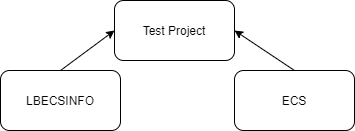
\includegraphics[scale = 0.5]{images/subsystem.png}
\end{center}
I have read a lot of the documentation about the distributed managements, and distributed systems.  I have learnt that you can configure them through an existing wizard only if you create a new project. Else you should do it via the configuration files. The Test Project configuration file should look like this :\newline
[general]\newline
distributed = 1\newline
[dist]\newline
distPeer = "dist\_name\_ECS" 1130\newline
distPeer = "dist\_name\_LBECSINFO" 1140\newline

I have tried to launch script from the copied project, but without any success, I haven't succeed to 



\normalsize
\end{document}